\documentclass{beamer}

\mode<presentation>
\usetheme{MarzStyle}
\graphicspath{{../images/}}

\usepackage[english]{babel}
\usepackage[scaled=.90]{helvet}
\usepackage{courier}

\begin{document}
	\author{Pascal Gerig, Lorenzo Wipfli, Marcel Zauder}
	\title{Can Crowd-Sourcing coexist with today's Data Security Regulations?}
	\institute{
\includegraphics[scale=1.5]{human-ist_logo.eps} \\ HUMAN-IST}
	\date{\today}

\begin{frame}
	\titlepage
\end{frame}

	\institute{HUMAN-IST}

%\AtBeginSection[]
%{
%  \begin{frame}<beamer>
%    \frametitle{Outline}{
%    	\tableofcontents[currentsection]
%    }
%  \end{frame}
%}

\begin{frame}{Background and Motivation}
	\begin{block}{Background}
		\begin{enumerate}[]
			\item Data collection by smart cities from population
		\end{enumerate}
	\end{block}
\end{frame}

\begin{frame}{Background and Motivation}
	\begin{block}{Background}
		\begin{tabular}{lc}
			\begin{tabular}{p{4.9cm}}
				\begin{enumerate}[]
					\item GDPR introduction in 2018
					\item Law enforcements impose hefty fines
				\end{enumerate}
			\end{tabular}
			&
			\begin{tabular}{c}
				\hfill \\ \vspace{0.3cm}
				
\includegraphics[scale=0.9]{GDPR.jpg}
			\end{tabular}
		\end{tabular}
	\end{block}
\end{frame}

\begin{frame}{Background and Motivation}
	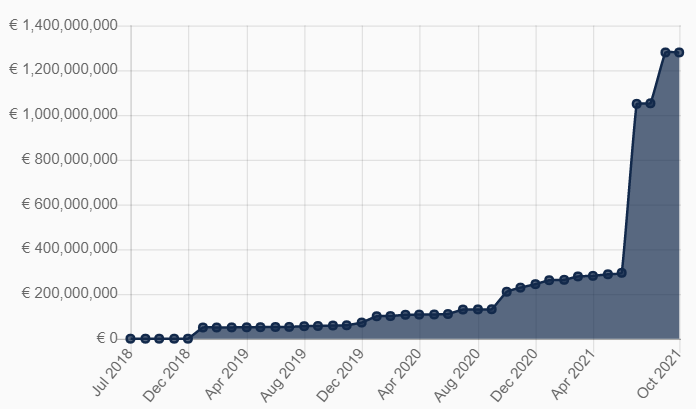
\includegraphics[scale=0.7]{EnforcementTracker_21-10-12.png}
\end{frame}

\begin{frame}{Background and Motivation}
	\begin{block}{Motivation}
		\begin{enumerate}[]
			\item Important to comply with new regulations (GDPR)
		\end{enumerate}
	\end{block}
	\begin{adjustwidth}{-2em}{}
		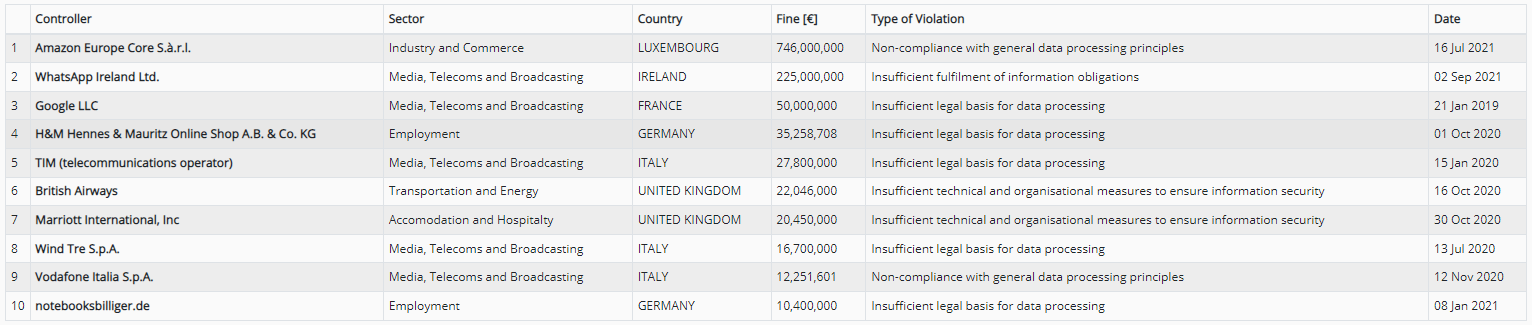
\includegraphics[scale=0.3]{Enforcement_Tracker_Fines.png}
	\end{adjustwidth}	
\end{frame}

\begin{frame}{Problem Statement and Research Question}
	\begin{block}{Research Question I}
		What methods do exist in order to gather information from citizen?
	\end{block}
\end{frame}

\begin{frame}{Problem Statement and Research Question}
	\vspace{1cm}
	\begin{block}{Research Question II}
		\begin{wrapfigure}{r}{0.5\textwidth}
			\vspace{-2cm} \hspace{-0.4cm}
			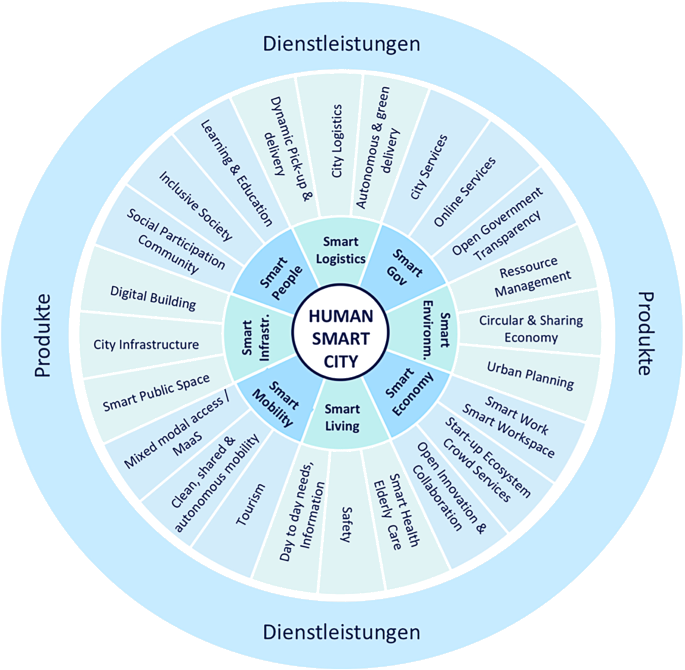
\includegraphics[width=1.2\linewidth]{Smart_City_Wheel_extended.png}
		\end{wrapfigure}
		What aspects do Human Smart Cities need to consider in order to comply with GDPR? \\
		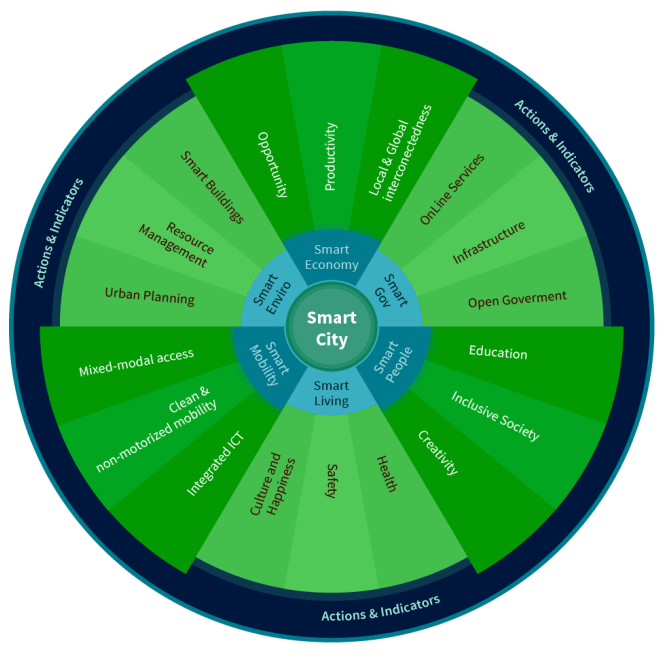
\includegraphics[scale=0.2]{Smart_City_Wheel.png}
	\end{block}
\end{frame}

\begin{frame}{Methodology}
	Following the Design Science Research principles
	\begin{block}{Artifact}
		Design principles and guidelines for designing crowd-sourcing methods
	\end{block}
	\begin{block}{Proceeding}
		\begin{enumerate}[]
			\item literature review
			\item design artifact
			\item descriptive artifact evaluation
		\end{enumerate}
	\end{block}
\end{frame}


\end{document}